\chapter{Анализ}\label{ch:ch2}

Данная глава описывает решения, которые были приняты для выполнения основной задачи данной ВКР.

\section{Анализ окружающего пространства}

По ходу анализа задачи данной ВКР было принято решение установить на будущего робота два основных сенсора, речь о которых шла в пункте~\ref{sec:environment-analysis}: это видеокамера и лазерный сканер, реализующий технологию Лидар\footnote{Лидар - технология получения и обработки информации об удалённых объектах при помощи активной оптической системы\cite[с. 20]{mather2005computer}.}.

Целью установки Лидара стала необходимость в сборе данных обо всём окружающем пространстве без необходимости совершать полный разворот. Такие данные можно было бы собирать и при помощи такого сенсора, как Xbox Kinect\footnote{Xbox Kinect - это бесконтактный сенсорный игровой контроллер, нашедший своё применение не только в игровой индустрии, но и в интерактивных экспозициях, и в робототехнике\cite{kinect-habr}.}, изображённого на Рисунке~\ref{fig:KinectSensor}, однако сбор информации об обстановке вокруг требовало бы полного оборота робота вокруг своей оси или установки сенсора на сервопривод. Разумеется, не во всех задачах роботу требуется видеть обстановку вокруг себя, в большинстве случаев роботу достаточно видеть то, что находится перед ним. Однако Лидар, в том числе, позволяет довольно быстро получать динамические данные вокруг робота. Это беусловно является преимуществом.
%https://ru.wikipedia.org/wiki/Kinect#/media/Файл:KinectSensor.png
\begin{figure}[ht]
  \centerfloat{
    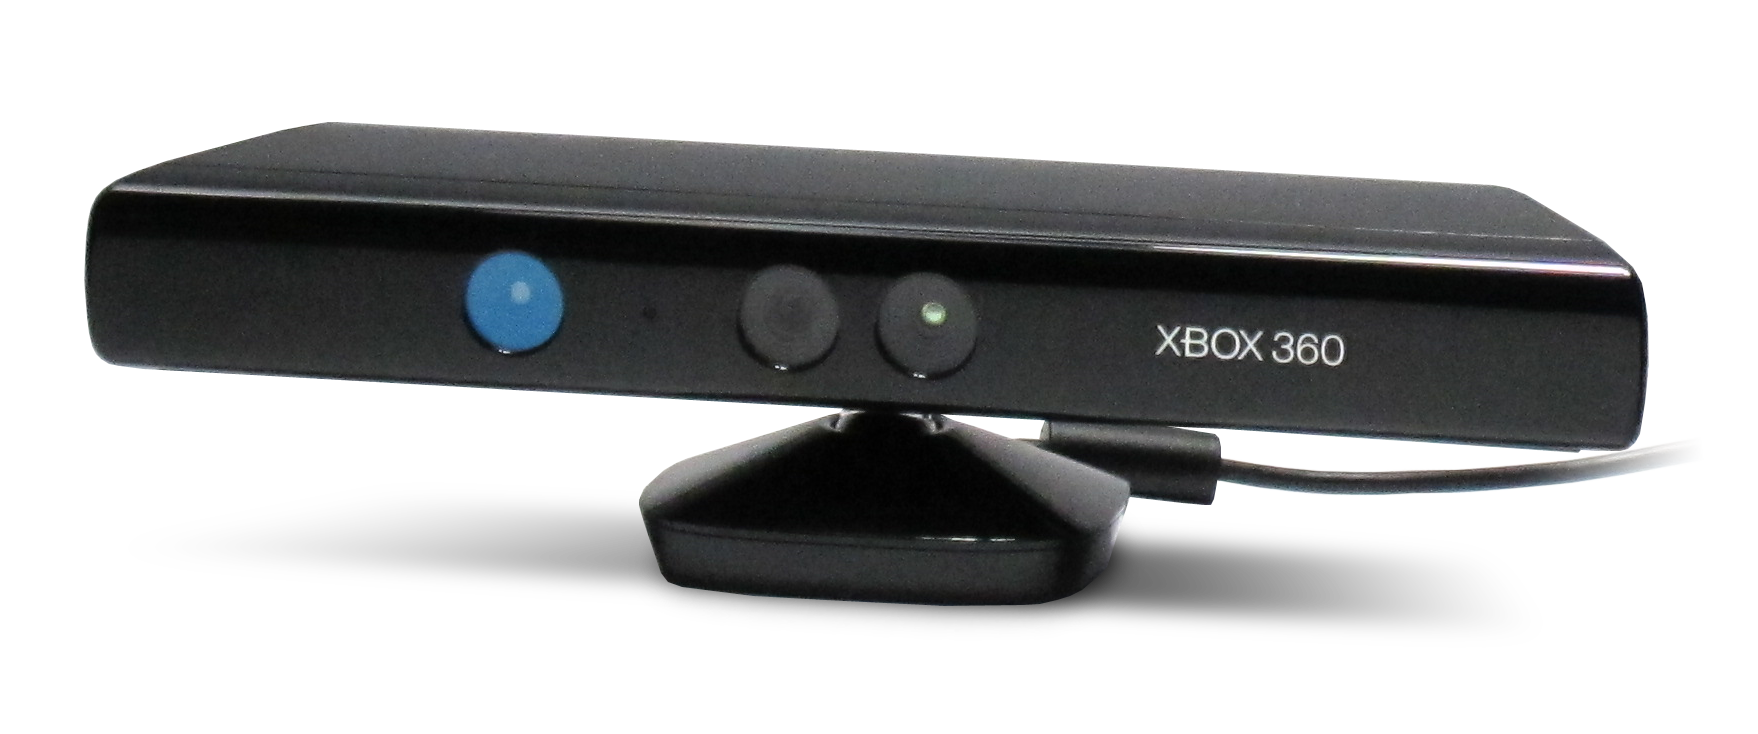
\includegraphics[scale=0.27]{KinectSensor.png}
  }
  \caption{Игровой сенсор Xbox Kinect, представленный в 2009 году в рамках выставки электронных развлечений E3.}\label{fig:KinectSensor}
\end{figure}

Целью установки видеокамеры является необходимость в выполнении роботом какой-то дополнительной полезной функции. В случае данной ВКР, в робот был встроен механизм поиска целевых объектов на окружающей местности.  

\section{Шасси и система управления}
В качестве шасси для робота был выбран вариант с гусеницами, так как это несло большую пользу в практическом плане: это не дорого и обладает преимуществами, которые были описаны в пункте~\ref{sec:about-driving}.
%\fixme{У робота должны быть передний ход, задний ход, управление гусеницами или колесами и т.д.}
Cистема управления шасси робота должна характеризоваться следующим:
\begin{enumerate}
\item Каждая гусеница управляется отдельно;
\item Возможность двигаться вперёд и назад;
\item Управляется простым логическим сигналом (1 - выполнять движение, 0 - не выполнять движение);
\item Программный интерфейс системы управления должен полностью раскрывать возможности аппаратной части.
\end{enumerate}

\section{Поведенческая стратегия робота}
В пункте~\ref{sec:robot-behavior} были описаны две возможные стратегии, которые можно применить на практике. Для облегчения задачи на данном этапе разработки было принято решение реализовать более лёгкую стратегию при которой поиск целевого объекта будет выполняться во время объезда пространства роботом. При этом карта местности всё же будет строиться и она будет служить для распознавания застревания робота, что очень важно при езде на неровных и мягких поверхностях.

Таким образом, поведенческая стратегия робота в данной ВКР сводится к тому, что робот в общем случае будет ехать вперёд и искать две вещи:
\begin{enumerate}
\item Преграду перед собой (распознаётся Лидаром);
\item Целевой объект (распознаётся видеокамерой);
\end{enumerate} 

В случае, если впереди была обнаружена преграда, то роботу уже не стоит ехать вперёд (так как он просто ударится), а найти какой-то другой путь. Самым логичным решением в данной ситуации станет поворот налево или направо. О том в какую сторону поворачивать, робот принимает решение на основе облака точек\footnote{Облако точек в данном конкретном случае будет представлять собой двумерный массив с числами типа float.}, которое предоставляет Лидар. В итоге поворот выполняется в ту сторону, где было найдено больше свободного пространства и меньше преград. Подробнее о том, как реализовано распознавание преград и свободного пространства будет описано в пункте~\ref{subsub:obstacle-avoidance}.

\section{Вычислительная составляющая}
К вычислительной составляющей мобильного автономного робота предъявляются довольно сильные и строгие требования:
\begin{itemize}
\item Компактность (для размещения на корпусе);
\item Мощность (требуется в реальном времени обрабатывать показания со всех сенсоров и выполнять движение);
\item Энергоэффективность (для большего времени автономной работы);
\item Бюджетность (в рамках данного проекта больших финансовых затрат не планировалось).
\end{itemize}

Было принято решение о том, что вычислительной составляющей будет одноплатный компьютер Nvidia Jetson NANO, изображённый на Рисунке \ref{fig:nvidia-jetson-nano}, так как он соответствует всем изложенным выше требованиям.

\begin{figure}[ht]
  \centerfloat{
    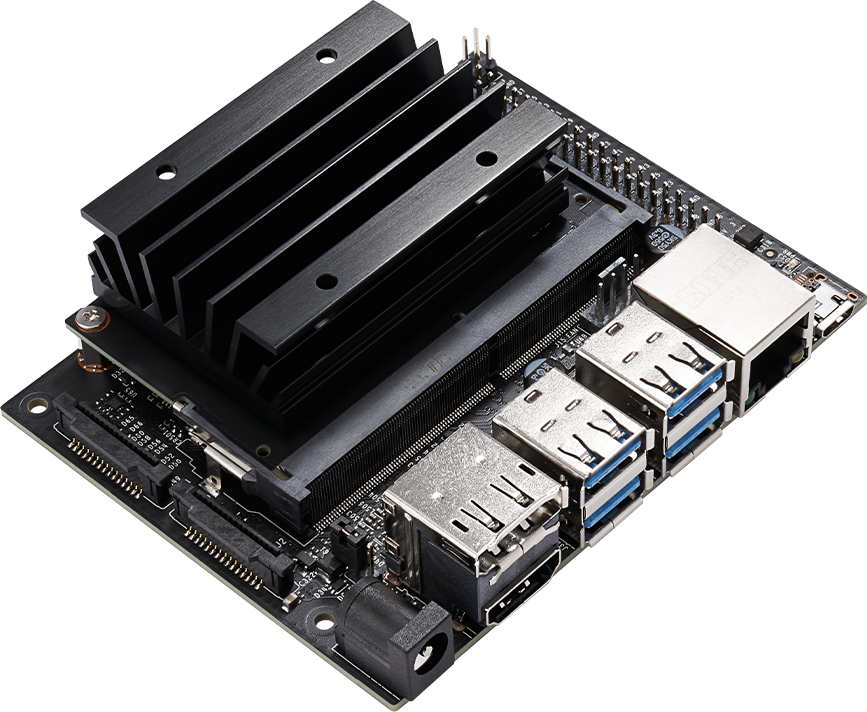
\includegraphics[scale=0.27]{nvidia-jetson-nano}
  }
  \caption{NVIDIA Jetson Nano - компактный и мощный одноплатный компьютер, представленный в 2019 году.}\label{fig:nvidia-jetson-nano}
\end{figure}

К основным характеристикам данного компьютера можно отнести следующие\cite{jetson-nano-overview}:
\begin{itemize}
\item Создан специально для встраиваемых систем;
\item Архитектура NVIDIA Maxwell™ с 128 ядрами NVIDIA CUDA®;
\item Четырехъядерный процессор ARM® Cortex®-A57 MPCore;
\item Размер 69,6 мм x 45 мм;
\item Имеет разъём GPIO и Ethernet.
\end{itemize}

\section{Известные аналоги}
К известным аналогам разрабатываемого робота, созданных на базе такого же одноплатного компьютера Nvidia Jetson NANO можно причислить роботов от самой компании Nvidia: Jetbot и Kaya. Оба эти робота были созданы для демонстрации возможностей данного одноплатного компьютера.

\subsection{Nvidia Kaya}
Данная модель компактного мобильного автономного робота была представлена на технологической конференции GTC 2019 и в первую очередь предназначается для работы с программным обеспечением Isaac SDK. Робот представлен на Рисунке~\ref{fig:kaya}.

\begin{figure}[ht]
  \centerfloat{
    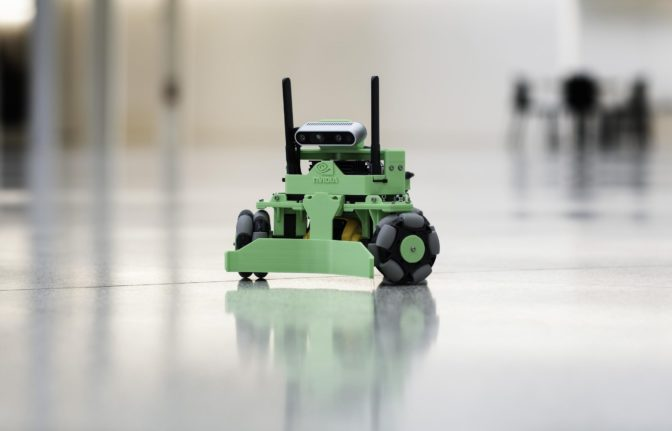
\includegraphics[scale=0.8]{kaya}
  }
  \caption{Внешний вид робота NVIDIA Kaya.}\label{fig:kaya}
\end{figure}

%https://docs.nvidia.com/isaac/isaac/doc/tutorials/assemble_kaya.html
%https://docs.nvidia.com/isaac/isaac/doc/tutorials/kaya_software.html
Аппаратно данный робот помимо самого Jetson NANO включает в себя пластиковый корпус на трёх колёсах (печатаемый на 3D принтере), 3D камеру LiDAR Intel Real Sense и систему управления. Общая стоимость аппаратной части на момент написания данной ВКР\footnote{Май 2020 г.} составляет \$812.87\cite{kaya-hardware}.

На компьютер Jetson NANO помимо ОС Ubuntu 18.04 LTS устанавливается ПО Isaac SDK и Isaac SIM. Isaac SDK - это открытая платформа NVIDIA для интеллектуальных роботов. Она предоставляет большой набор мощных алгоритмов, базирующихся на GPU вычислениях\footnote{вычисления на видеокарте} для навигации и управления.

На данном роботе можно запускать различные готовые примеры такие как ручное управление с геймпада Playstation 4, автономное следование за AprilTag, распознавание объектов на нейронной сети DetectNetv2 и алгоритм SLAM (основан на GMapping)\cite{kaya-software}.

\subsection{Nvidia JetBot}
JetBot был представлен на той же конференции, что Nvidia Kaya и является гораздо более доступным вариантом (цена \$226.15) для создания DIY робота (также он в отличии от Kaya имеется в розничной продаже одним комплектом и его не нужно собирать по частям из разных магазинов). Nvidia JetBot изображён на Рисунке~\ref{fig:jetbot-waveshare}\cite{jetbot-shop}.

\begin{figure}[ht]
  \centerfloat{
    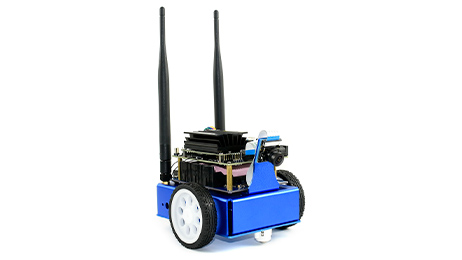
\includegraphics[scale=0.8]{jetbot-waveshare}
  }
  \caption{Набор инструментов NVIDIA JetBot от Waveshare.}\label{fig:jetbot-waveshare}
\end{figure}


Аппаратно он состоит из всё той же Nvidia Jetson Nano, двух электромоторов с драйвером в комплекте и CSI видеокамеры Sony IMX219.

Программная часть поставляется готовым образом на базе Ubuntu 18.04 в формате ISO для прошивки MicroSD карты.

Из доступных примеров имеется простое ручное управление через кнопки на экране с возможностью прямой трансляции изображения видеокамеры на экран в браузере и нейросеть, автономное движение по поверхности с распознанием препятствий и пропастей в окружающем пространстве при помощи нейросети на основе получаемого видеосигнала, также имеется функция следования робота за определённым целевым объектом\cite{jetbot-examples}.

\subsection{Сравнение с аналогами}
Робот, разрабатываемый в рамках данной ВКР по большей части сходится с Nvidia JetBot, однако подход к решению задач в корне изменён. Стратегия движения робота в данной ВКР полностью определяется показаниями Лидара, что даёт большую гибкость за счёт того, что Лидар сканирует всю поверхность вокруг себя тогда как видеокамера позволяет видеть только то, что находится непосредственно перед роботом. Таким образом робот, создаваемый в рамках данной ВКР решает уже решённую задачу другим более гибким способом.

Что касается Nvidia Kaya, то данная модель хоть и оснащена Лидаром, но обладает довольно большим минусом в виде цены за данный продукт. Также установленный там Лидар не может просматривать пространство вокруг себя в силу того что Лидаром является видеокамера, поворот которой занимает гораздо дольше времени по сравнению с лазерным сканером.

\FloatBarrier
